\documentclass[10pt, a4paper,spanish]{article}

\usepackage{./mystyle}
\usepackage{./myvars}



%-----------------------------

\begin{document}

	\maketitle % Insert title

	\thispagestyle{fancy} % All pages have headers and footers


%-----------------------------
%	ABSTRACT
%-----------------------------

	\begin{abstract}
		\noindent Abstract
	\end{abstract}

%-----------------------------
%	TEXT
%-----------------------------


  \section{Tómese la siguiente función lógica y obténgase el árbol de decisión correspondiente usando WEKA}

		\begin{equation}
			\label{eq:logic_equation}
			\neg(A \land B) \lor \neg(C \land D) \oplus E
		\end{equation}

		\begin{table}[p]
			\begin{center}
				\csvautotabular{data.csv}
			\end{center}
			\caption{Tabla de verdad de la ecuación \ref{eq:logic_equation}}
			\label{eq:truth_table}
		\end{table}


		\begin{figure}[h]
			\begin{center}
				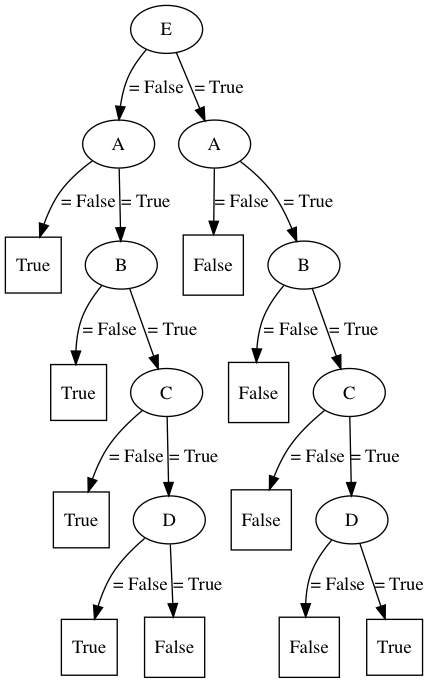
\includegraphics[width=0.5\textwidth]{id3-tree}
			\end{center}
			\caption{}
			\label{}
		\end{figure}

		\begin{figure}[h]
			\begin{center}
				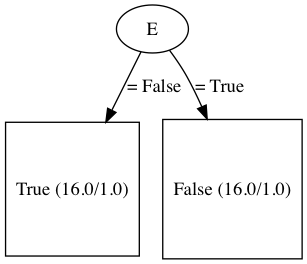
\includegraphics[width=0.5\textwidth]{j48-tree}
			\end{center}
			\caption{}
			\label{}
		\end{figure}

    \paragraph{}
		Prueba.

		\paragraph{}
		Las figuras han sido generadas\cite{github:ismtabo-treetograph}

		\paragraph{}
		Función lógica \cite{github:garciparedes-python-examples}

%-----------------------------
%	Bibliographic references
%-----------------------------
	\nocite{subject:taa}
  \bibliographystyle{acm}
  \bibliography{bib/misc}

\end{document}
